%%=============================================================================
%% Inleiding
%%=============================================================================

\chapter{\IfLanguageName{dutch}{Inleiding}{Introduction}}%
\label{ch:inleiding}

%\begin{itemize}
%  \item context, achtergrond
%  \item afbakenen van het onderwerp
%  \item verantwoording van het onderwerp, methodologie
%  \item probleemstelling
%  \item onderzoeksdoelstelling
%  \item onderzoeksvraag
%  \item \ldots
%\end{itemize}

\section{\IfLanguageName{dutch}{Probleemstelling}{Problem Statement}}%
\label{sec:probleemstelling}

Een sedentaire job wordt geassocieerd met schadelijke gevolgen voor de algemene gezondheid \autocite{Buckley2015}. Het is dus van groot belang dat voldoende beweging een prioriteit is.

\textcite{Hallal2012} beschouwen 31,1\% van de wereldwijde bevolking als inactief. Dit wil zeggen dat, op het moment van dit onderzoek, bijna een derde van de volwassen wereldbevolking de vooropgestelde aanbevelingen van de ``World Health Organization'' (WHO), beschreven door \textcite{Bull2020}, niet haalt. Voor Europa ligt deze waarde zelfs op 34,8\% en België ligt nog een stuk boven de gemiddelde Europese waarde met 40\% à 49,9\% (zie figuur \ref{fig:inactivity_inleiding}).

\begin{figure}[h]
    \caption[Fysieke inactiviteit bij volwassenen wereldwijd]{Fysieke inactiviteit volwassenen (15+) wereldwijd, bij mannen (A) en vrouwen (B) \autocite{Bull2020}.}
    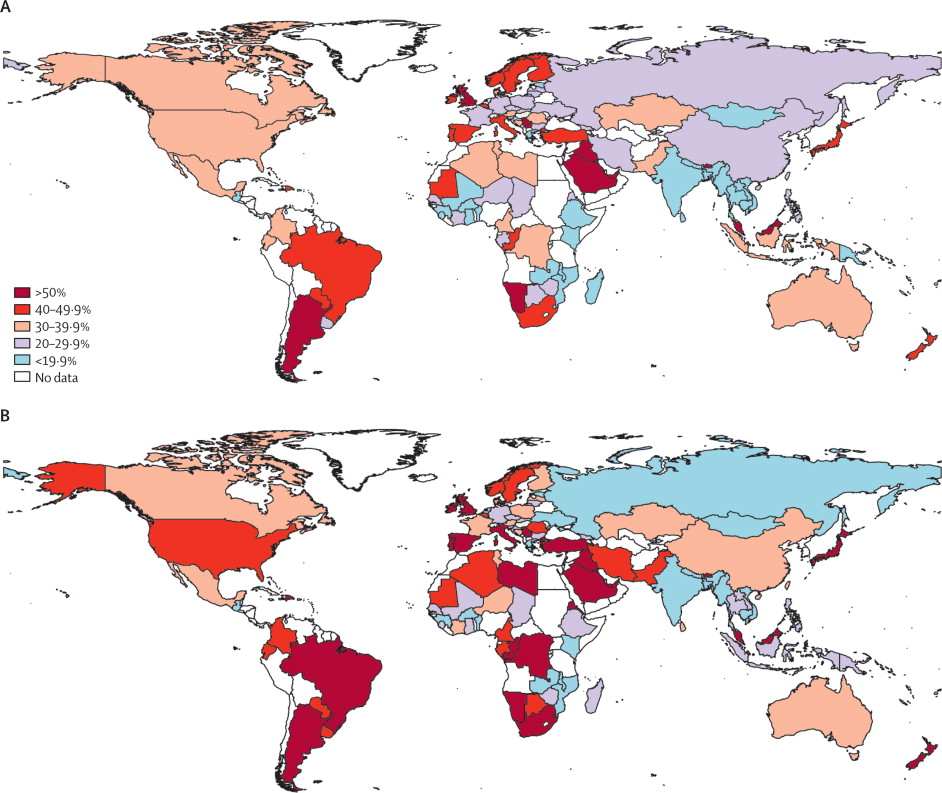
\includegraphics[width=1\textwidth]{Inactiviteit}
    \label{fig:inactivity_inleiding}
\end{figure}

Concreet zal deze paper bij (een deel van de) werknemers van \href{https://en.joule.be/}{Joule}, \href{https://www.ventures4growth.com/en}{Ventures 4 Growth}, \href{https://www.mace-legal.com/}{mace}, \href{https://planetb.life/en}{PlanetB}, \href{https://www.we-are.be/}{we are} en \href{https://www.delaware.pro/en-be}{delaware}, die allen een sedentaire job beoefenen, onderzoeken hoe het beweeggedrag is, en of een competitief sportplatform hen kan helpen de vooropgestelde hoeveelheden van de WHO te behalen.

%Uit je probleemstelling moet duidelijk zijn dat je onderzoek een meerwaarde heeft voor een concrete doelgroep. De doelgroep moet goed gedefinieerd en afgelijnd zijn. Doelgroepen als ``bedrijven,'' ``KMO's'', systeembeheerders, enz.~zijn nog te vaag. Als je een lijstje kan maken van de personen/organisaties die een meerwaarde zullen vinden in deze bachelorproef (dit is eigenlijk je steekproefkader), dan is dat een indicatie dat de doelgroep goed gedefinieerd is. Dit kan een enkel bedrijf zijn of zelfs één persoon (je co-promotor/opdrachtgever).

\section{\IfLanguageName{dutch}{Onderzoeksvraag}{Research question}}%
\label{sec:onderzoeksvraag}

%Wees zo concreet mogelijk bij het formuleren van je onderzoeksvraag. Een onderzoeksvraag is trouwens iets waar nog niemand op dit moment een antwoord heeft (voor zover je kan nagaan). Het opzoeken van bestaande informatie (bv. ``welke tools bestaan er voor deze toepassing?'') is dus geen onderzoeksvraag. Je kan de onderzoeksvraag verder specifiëren in deelvragen. Bv.~als je onderzoek gaat over performantiemetingen, dan

Deze paper zal onderzoeken of een competitief sportplatform, dat gebruik maakt van gamification, een positieve invloed kan hebben op het sportgedrag van personen in een sedentaire job. Daarnaast zal het ook achterhalen welke gamificationtechnieken  het meeste succes hebben, en of er technieken zijn die een negatief effect hebben.

\section{\IfLanguageName{dutch}{Onderzoeksdoelstelling}{Research objective}}%
\label{sec:onderzoeksdoelstelling}

Om deze problematiek te proberen verhelpen, zal een sportplatform ontwikkeld worden. Deze ``Proof Of Concept'' (POC) zal het onderzoek faciliteren naar hoe gamification mensen in een sedentaire job kan helpen meer te bewegen in hun dagelijks leven. Gamification is in de literatuur beschreven als het gebruiken van spelelementen die niet aan een spel gerelateerd zijn \autocite{Gaalen2020}. Het gebruik van deze elementen zorgt dan voor een bepaalde competitie.

%Wat is het beoogde resultaat van je bachelorproef? Wat zijn de criteria voor succes? Beschrijf die zo concreet mogelijk. Gaat het bv.\ om een proof-of-concept, een prototype, een verslag met aanbevelingen, een vergelijkende studie, enz.

\section{\IfLanguageName{dutch}{Opzet van deze bachelorproef}{Structure of this bachelor thesis}}%
\label{sec:opzet-bachelorproef}

De rest van deze bachelorproef is als volgt opgebouwd:

In Hoofdstuk~\ref{ch:stand-van-zaken} wordt een overzicht gegeven van de stand van zaken binnen het onderzoeksdomein, op basis van een literatuurstudie.

In Hoofdstuk~\ref{ch:methodologie} wordt de methodologie toegelicht en worden de gebruikte onderzoekstechnieken besproken om een antwoord te kunnen formuleren op de onderzoeksvragen.

In Hoofdstuk~\ref{ch:proofofconcept} worden de gekozen technologieën van de POC toegelicht en wordt de opbouw van de applicatie besproken.

In Hoofdstuk~\ref{ch:analyse} worden de cijfers geanalyseerd die uit zowel de bevragingen als de website komen.

In Hoofdstuk~\ref{ch:conclusie}, tenslotte, wordt de conclusie gegeven en een antwoord geformuleerd op de onderzoeksvragen. Daarbij wordt ook een aanzet gegeven voor toekomstig onderzoek binnen dit domein.